%%%%%%%%%%%%%%%%%%%%%%%%%%%%%%%%%%%%%%%%%
% LaTeX Template
% http://www.LaTeXTemplates.com
%
% Original author:
% Linux and Unix Users Group at Virginia Tech Wiki 
% (https://vtluug.org/wiki/Example_LaTeX_chem_lab_report)
%
% License:
% CC BY-NC-SA 3.0 (http://creativecommons.org/licenses/by-nc-sa/3.0/)
%
%%%%%%%%%%%%%%%%%%%%%%%%%%%%%%%%%%%%%%%%%

%----------------------------------------------------------------------------------------
%	PACKAGES AND DOCUMENT CONFIGURATIONS
%----------------------------------------------------------------------------------------

\documentclass[11pt]{article}
\usepackage{geometry} % Pour passer au format A4
\geometry{hmargin=1cm, vmargin=1cm} % 

\usepackage{graphicx} % Required for including pictures
\usepackage{float} % 

%Français
\usepackage[T1]{fontenc} 
\usepackage[english,francais]{babel}
\usepackage[utf8]{inputenc}
\usepackage{eurosym}
\usepackage{lmodern}
\usepackage{url}
\usepackage{multicol}

%Maths
\usepackage{amsmath,amsfonts,amssymb,amsthm}
%\usepackage[linesnumbered, ruled, vlined]{algorithm2e}
%\SetAlFnt{\small\sffamily}

%Autres
\linespread{1} % Line spacing
\setlength\parindent{0pt} % Removes all indentation from paragraphs

\renewcommand{\labelenumi}{\alph{enumi}.} % 
\pagestyle{empty}
%----------------------------------------------------------------------------------------
%	DOCUMENT INFORMATION
%----------------------------------------------------------------------------------------
\begin{document}

%\maketitle % Insert the title, author and date

\setlength{\columnseprule}{1pt}

\section{I - $f(x) = 0.5x^2 - 5x +1$}
\begin{figure}[H]
  \centering
  
\includegraphics[width=0.6\textwidth]{sources/exo/grid.png}
\end{figure}

\begin{center}
  \begin{tabular}{| c | c | c | c | c | c | c | c | c | }
    \hline
    $x$    & -2               & 0                & 2                & 4                & 6                & 8                & 10               & 12\\
    \hline
    $f(x)$ & \phantom{123456} & \phantom{123456} & \phantom{123456} & \phantom{123456} & \phantom{123456} & \phantom{123456} & \phantom{123456} & \phantom{123456} \\
    \hline
    $f'(x)$ & \phantom{123456} & \phantom{123456} & \phantom{123456} & \phantom{123456} & \phantom{123456} & \phantom{123456} & \phantom{123456} & \phantom{123456} \\
    \hline
  \end{tabular}
\end{center}

\section{II - $g(x) = x^3 - 5x^2 + 2x + 4$}

\begin{figure}[H]
  \centering
  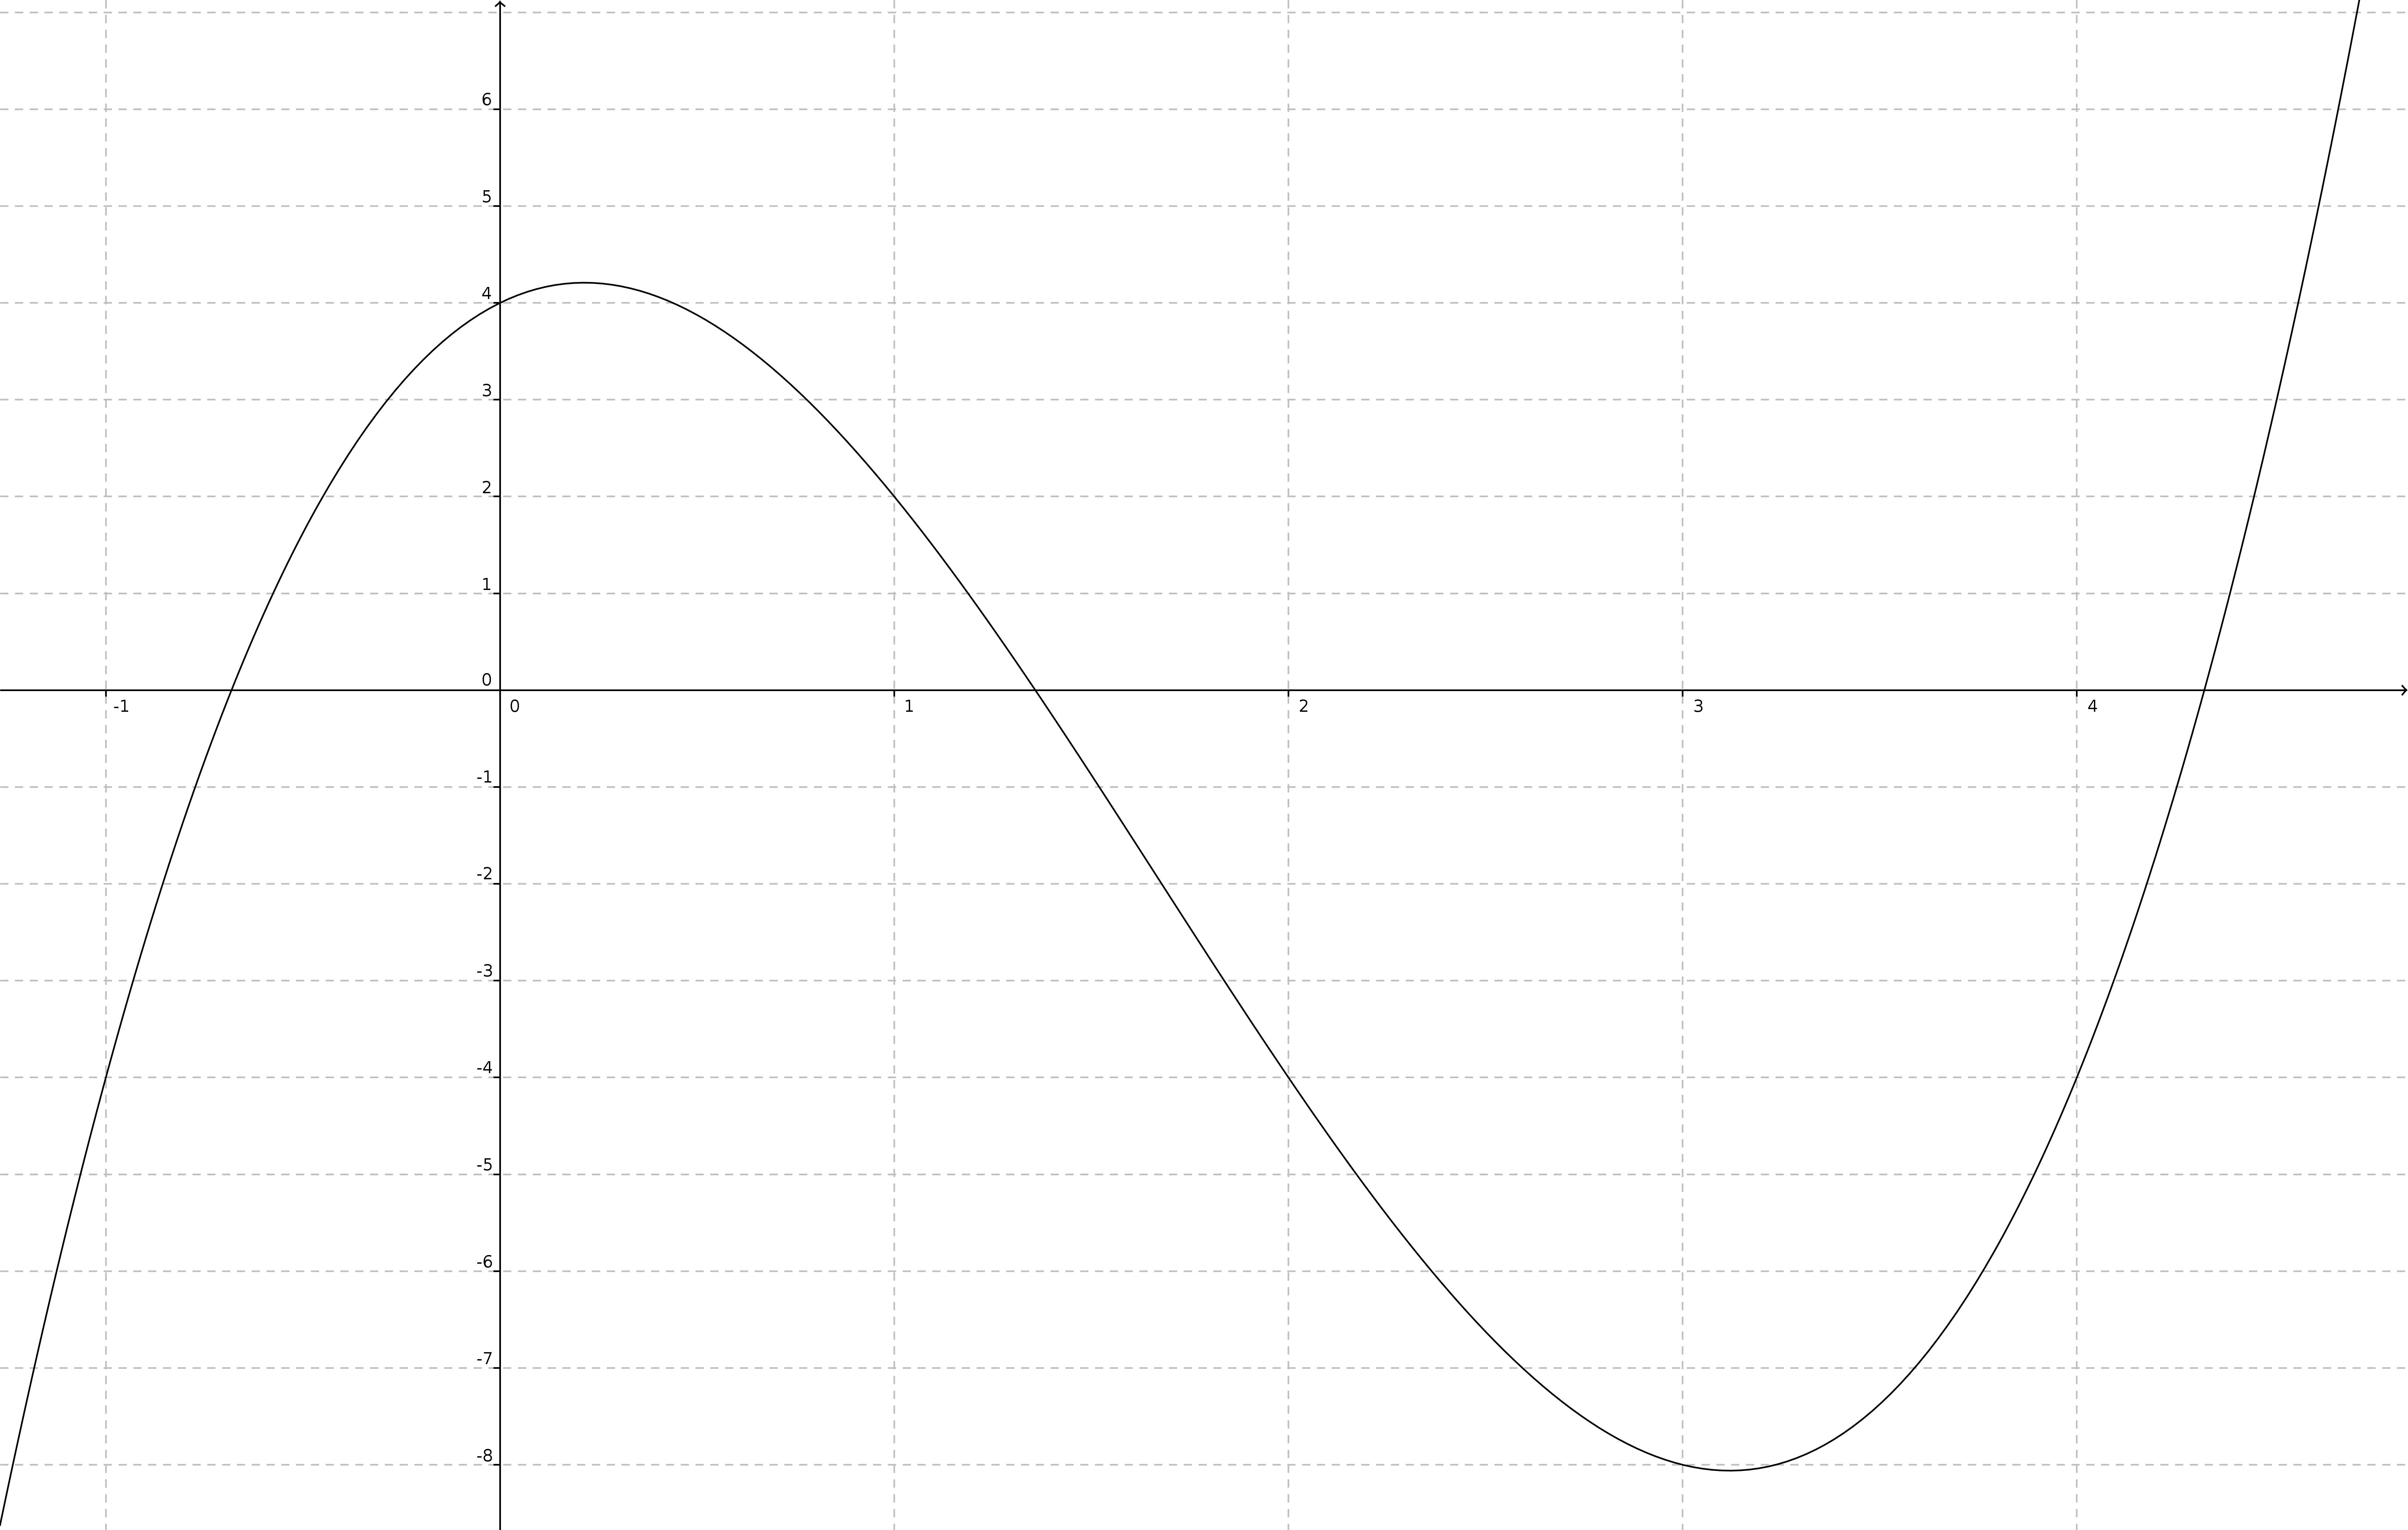
\includegraphics[width=0.6\textwidth]{sources/exo/grid2.png}
\end{figure}

\begin{center}
  \begin{tabular}{| c | c | c | c | c | c | c | }
    \hline
    $x$     & -1               & 0                & 1                & 2                & 3                & 4\\
    \hline
    $g(x)$  & \phantom{123456} & \phantom{123456} & \phantom{123456} & \phantom{123456} & \phantom{123456} & \phantom{123456} \\
    \hline
    $g'(x)$ & \phantom{123456} & \phantom{123456} & \phantom{123456} & \phantom{123456} & \phantom{123456} & \phantom{123456}  \\
    \hline
  \end{tabular}
\end{center}

\begin{enumerate}
\item Remplir la ligne $f(x)$ du tableau.
\item Placer les points sur le graphique puis les relier.
\item Tracer les tangentes et lire leurs coefficients directeurs afin de remplir la ligne $f'(x)$
\item Placer les points $(x ; f'(x))$ sur le graphique et relier les points.
\item En déduire la fonction $f'(x)$.
\end{enumerate}

\end{document}
